%\sectcounter{subsection}{2}
\subsection{Introduction}

%\section{Exploiter les données enregistrées sur le système Comax}
Dans cette partie, on va s’appuyer\emph{•} sur un support de TP qui est utilisé aux oraux de concours : le système CoMax présenté sur la figure 1. Ce système est une adaptation pédagogique de la solution industrielle ZE de SAPELEM. Le principe de fonctionnement de ces deux systèmes repose sur l’utilisation d’un système de levage motorisé, associé à une poignée, équipée d'un capteur d’effort (voir Figure~\ref{sys_comax}).

\begin{figure}[!h]
\centering
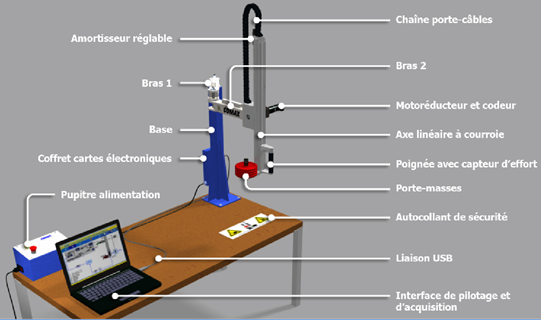
\includegraphics[width=0.8\textwidth]{image/sys_comax.png}
\caption{Présentation du système Comax}
\label{sys_comax}
\end{figure}

\subsection{Extraction des données expérimentales}
Nous allons dans cette partie utiliser les résultats d’expérimentions sur le robot CoMax. Ces résultats sont fournis dans le fichier \textit{CoMax.txt}. Ils correspondent à un fichier brut avec les points de mesures expérimentales. 


\vspace{5mm}
\question{Après avoir observé la structure du fichier \textit{CoMax.txt}, proposer des instructions permettant d'extraire sous deux listes distinctes \texttt{temps} et \texttt{q\_exp} les instants de prise d'échantillonnage et les positions codeur correspondantes en tops (nombre de points). Ces deux listes seront converties en tableaux Numpy (\texttt{import numpy as np}), grâce à la commande \texttt{liste=np.array(liste)}.}

\vspace{5mm}
La position de l'axe linéaire $X(t)$ [en mm] est liée à la position du moteur $q_m$ [en tops] renvoyée par le codeur selon la formule suivante : $X = \dfrac{3,41.q_m}{1000}$ 

\vspace{5mm}
\question{Générer alors un tableau des positions verticales de l'axe nommé \texttt{X\_exp}, qui a une condition initiale nulle sur la position.}

\vspace{5mm}
\question{Tracer l'évolution des positions mesurées expérimentales en fonction du temps, avec des croix bleues (+). On légendera correctement les axes, et on indiquera une légende du type : "points mesurés"}

\subsection{Étude des performances attendues du système}
Dans un second temps, nous allons modéliser le comportement attendu système. La modélisation du système est faite en amont du système réel, lors de la phase de conception, mais elle est importante pour comprendre un système réel afin de proposer des modifications affectant les performances.

Les réponses attendues en vitesse V(t) et en position X(t) de l’axe linéaire sont représentées en Figure~\ref{lois_horaires} . Les caractéristiques de la loi en vitesse sont les suivantes :
\begin{itemize}
\item l’instant de début de mouvement : $t_0=0 s$ ;
\item la position initiale et la vitesse initiale : $X(0)=X_0=0 m$ et $V(0)=0 m/s$;
\item l’accélération : $A_{cmax}=2,83 m/s^2$ ;
\item la vitesse maximale : $V_{max}=0,68 m/s$.
\end{itemize}

\begin{figure}[!h]
\centering
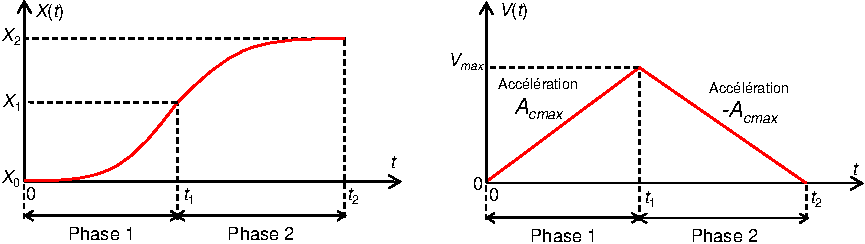
\includegraphics[width=0.9\textwidth]{image/lois_horaires.pdf}
\caption{Lois d'évolution en position (à gauche) et en vitesse (à droite) du CoMax}
\label{lois_horaires}
\end{figure}

On peut montrer par intégration successives, en tenant compte des conditions initiales que :

\vspace{0.5cm}
\begin{tabular}{|l|l|l|}
    \hline
     \textbf{Phase} &  \textbf{1} & \textbf{2}  \\
    \hline
     instant $t$  & $0\leq t <t_1$ & $t_1 \leq t \leq t_2$ \\
    \hline
     accélération $A(t)$  & $A_{cmax}$ & $-A_{cmax}$ \\
    \hline
     vitesse $V(t)$  & $A_{cmax}.t$ & $V_{max}-A_{cmax}.(t-t_1)$ \\
    \hline
     position $X(t)$  & $\dfrac{1}{2}.A_{cmax}.t^2$ & $X_1 + V_{max}.(t-t_1) - \dfrac{1}{2}.A_{cmax}.(t-t_1)^2$  \\
    \hline
\end{tabular}

On notera que : $X_1 = X(t_1)$, à l'issue de la phase 1 et $X_2=X(t_2)$, à l'issue de la phase 2.

\vspace{0.5cm}
\question{Trouver les expressions littérales de $t_1$, $t_2$, $X_1$ et de $X_2$ en fonction de $A_{cmax}$ et de $V_{max}$.}

\vspace{0.5cm}
\question{Concevoir deux fonctions \texttt{Loi\_Vitesse} et \texttt{Loi\_position} prenant en argument un instant $t$ et permettant de retourner la vitesse, respectivement la position, à cet instant. (A noter que l'on pourra introduire des variables globales, comme $t_1$, $t_2$, etc.)}

\vspace{0.5cm}
On rappelle que la commande \texttt{y = np.zeros(n)} permet de générer un tableau de taille $n \times 1$ contenant des 0.  

\vspace{0.5cm}
\question{Construire deux tableaux \texttt{X\_th} et \texttt{V\_th} où sont stockées les positions théoriques commandées, respectivement vitesses théoriques aux instants définis dans le tableau \texttt{temps}. Superposer la courbe d'évolution de la position théorique sur les points expérimentaux, obtenus précédemment (tracé en vert, ligne continue, avec légende explicite). Sur une nouvelle figure tracer en vert, trait continu, l'évolution de la vitesse théorique}.


\subsection{Quantification et analyse des écarts}

Nous allons quantifier l’écart de performance entre l’exigence du cahier des charges et le système réel. Pour cela, nous allons calculer les écarts et utiliser des outils de statistique pour quantifier ces écarts.

On définit l'écart relatif en \% $\delta_\%$ entre une valeur théorique $x_{th}$ et une valeur expérimentale $x_{exp}$ : $\delta_\%=\displaystyle\left\lvert  \dfrac{x_{exp}-x_{th}}{x_{th}} \right\rvert$ 

\vspace{0.5cm}
\question{Concevoir une fonction \texttt{Calcul\_ecarts} prenant en arguments deux tableaux à une dimension et retournant un tableau \texttt{Delta\_X} de même dimension où sont stockés les écarts relatifs entre chacune des valeurs des deux tableaux spécifiés en arguments d'entrée.}

\vspace{0.5cm}
\question{Tracer un histogramme montrant l'évolution des écarts relatifs en position en fonction du numéro de la mesure (on utilisera \texttt{plt.bar} et \texttt{plt.subplot}). On n'évaluera pas l'écart relatif sur la première valeur (nulle).}

\vspace{0.5cm}
On rappelle ici quelques notions de statistiques :
\begin{itemize}
    \item La médiane d'un ensemble de valeurs (échantillon, population, distribution de probabilités) est une valeur qui partage la série en deux parties de même effectif.
    \item L’écart type est défini comme la moyenne quadratique des écarts par rapport à la moyenne. Il a la même dimension que la variable statistique étudiée.
\end{itemize}

\vspace{0.5cm}
\question{Écrire une fonction \texttt{Calculs\_stats} permettant, à partir d'un tableau \texttt{T} passé en argument, de retourner un tuple de 3 valeurs : moyenne, médiane et écart type. \textit{Indication :} On pourra utiliser les fonctions de la bibliothèque numpy (\texttt{np.sum(T)}, pour faire la somme de tous les éléments du tableau \texttt{T}, \texttt{np.sort(T)}, pour trier le tableau \texttt{T} dans l'ordre croissant. Appliquer le résultat au tableau \texttt{Delta\_X}.}

\vspace{0.5cm}
\question{Comparer les résultats en utilisant les fonctions suivantes : \texttt{np.mean}, pour la moyenne ; \texttt{np.median}, pour la médiane et \texttt{np.std}, pour l'écart type}
\label{LastPage}
\end{document}